\subsection{Diagramas de casos de uso}
\begin{figure}[H]
    \centering
    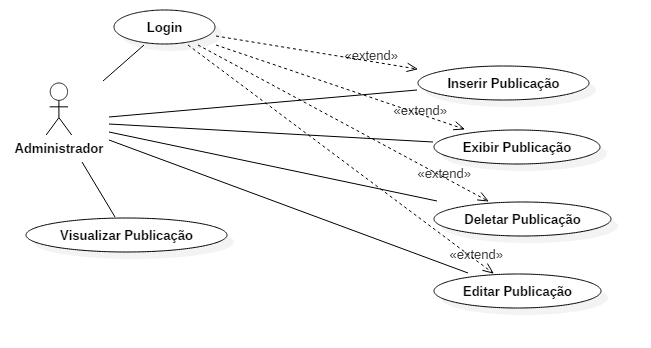
\includegraphics[width=\textwidth]{figuras/casosDeUsoADM}
    \caption{Diagrama de casos de uso do módulo administrador}
\end{figure}

\begin{figure}[H]
    \centering
    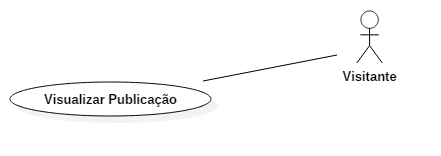
\includegraphics[width=\textwidth]{figuras/CasosDeUsoCliente}
    \caption{Diagrama de casos de uso do módulo cliente}
\end{figure}

\begin{figure}
    \centering
    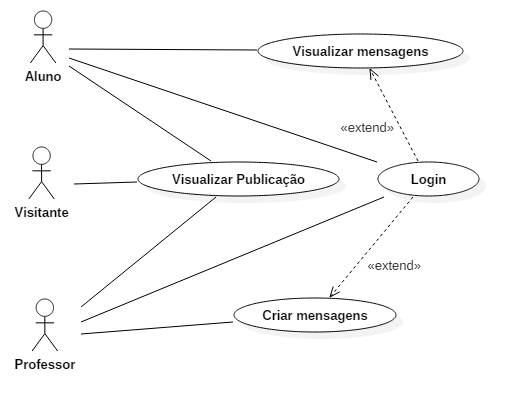
\includegraphics[width=\textwidth]{figuras/CasosDeUsoMobile}
    \caption{Diagrama de casos de uso do aplicativo móvel}
\end{figure}

\subsection{Diagramas de classe}
\begin{figure}[H]
    \centering
    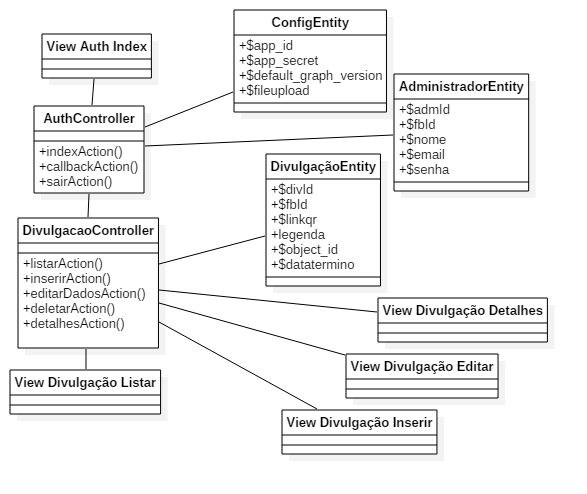
\includegraphics[width=\textwidth]{figuras/diagramaclasseADM}
    \caption{Diagrama de classes do módulo administrador}
\end{figure}

\begin{figure}[H]
    \centering
    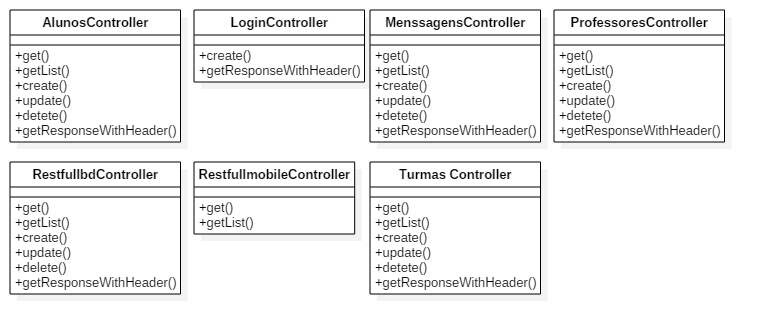
\includegraphics[width=\textwidth]{figuras/diagramaclasseAPI}
    \caption{Diagrama de classes do submódulo API}
\end{figure}

\begin{figure}[H]
    \centering
    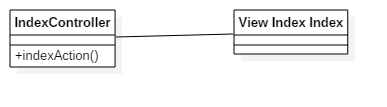
\includegraphics[width=\textwidth]{figuras/diagramaclasseCLIENTE}
    \caption{Diagrama de classes do módulo Cliente}
\end{figure}

\subsection{Diagramas entidade--relacionamento}
\begin{figure}[H]
    \centering
    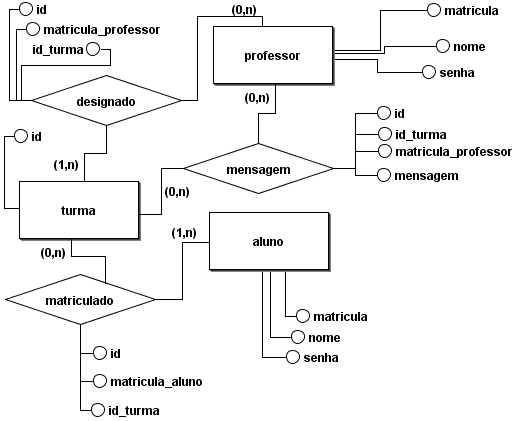
\includegraphics[width=\textwidth]{figuras/entidaderelacionamentomobile}
    \caption{Diagrama entidade--relacionamento do aplicativo móvel (API fictícia)}
\end{figure}

\begin{figure}[H]
    \centering
    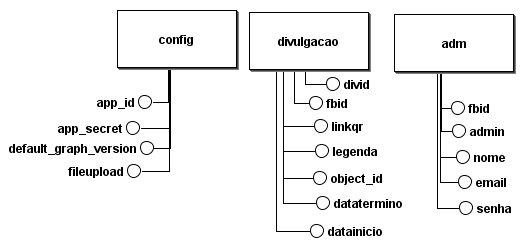
\includegraphics[width=\textwidth]{figuras/entidaderelacionamento}
    \caption{Diagrama entidade--relacionamento do \textit{web}}
\end{figure}

\subsection{Diagramas de sequência}
\begin{figure}[H]
    \centering
    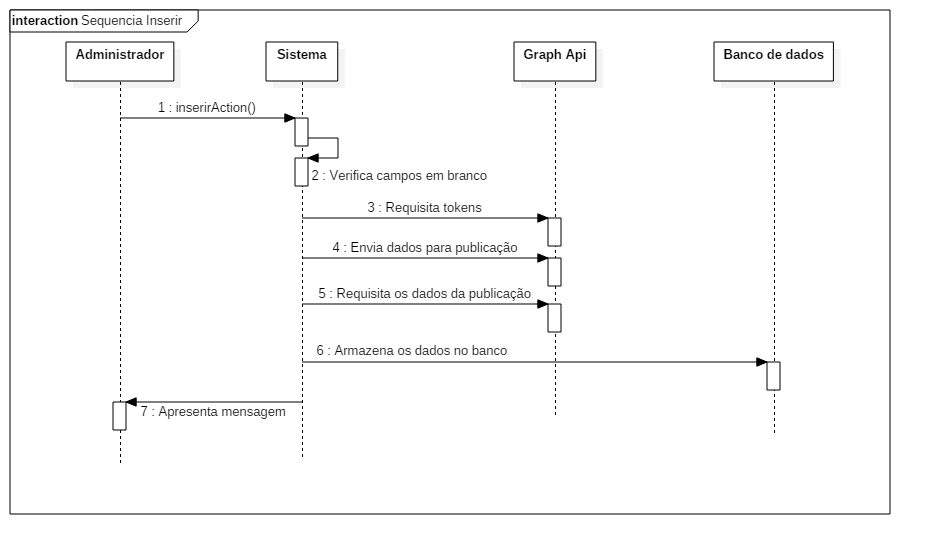
\includegraphics[width=\textwidth]{figuras/sequenciainserir}
    \caption{Diagrama de sequência para inserir}
\end{figure}

\begin{figure}[H]
    \centering
    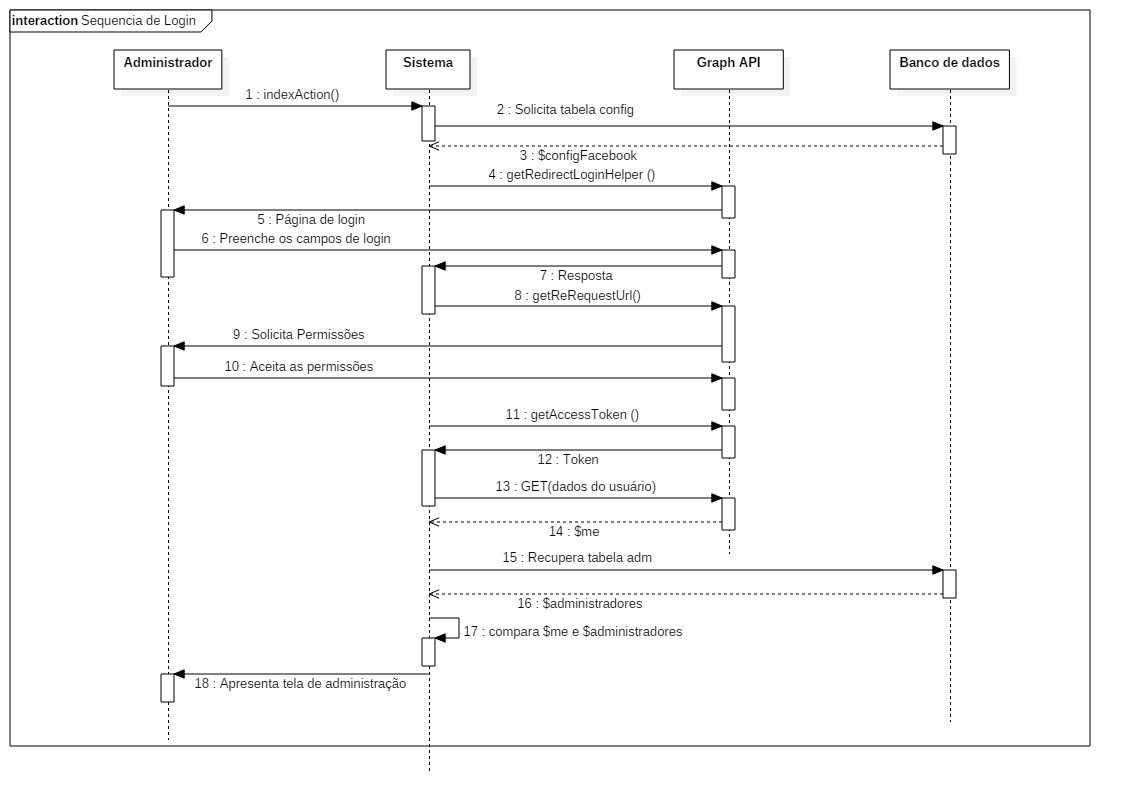
\includegraphics[width=\textwidth]{figuras/sequencialogin}
    \caption{Diagrama de sequência para login}
\end{figure}

\begin{figure}[H]
    \centering
    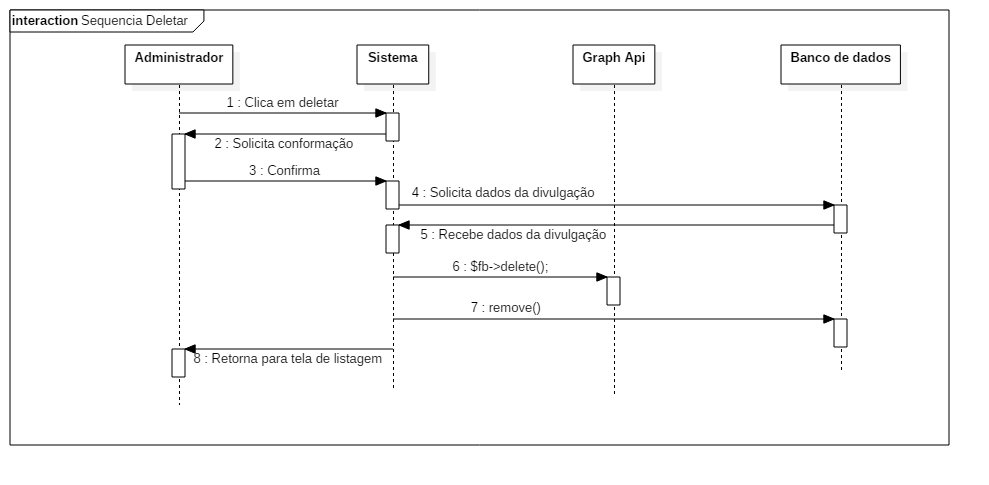
\includegraphics[width=\textwidth]{figuras/sequenciaDeletar}
    \caption{Diagrama de sequência para deletar}
\end{figure}

\begin{figure}[H]
    \centering
    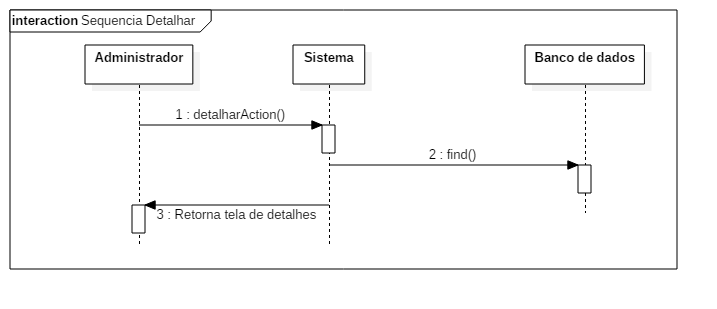
\includegraphics[width=\textwidth]{figuras/sequenciaDetalhar}
    \caption{Diagrama de sequência para detalhar}
\end{figure}

\begin{figure}[H]
    \centering
    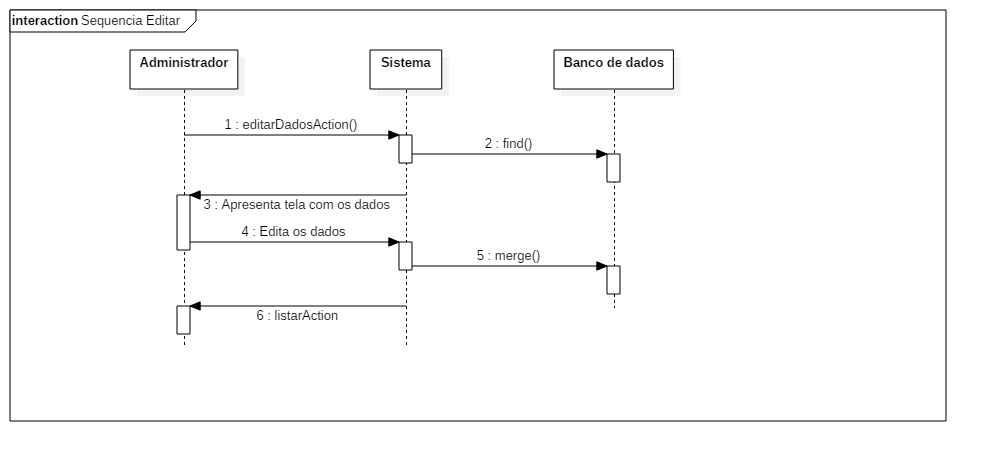
\includegraphics[width=\textwidth]{figuras/sequenciaEditar}
    \caption{Diagrama de sequência para editar}
\end{figure}

\begin{figure}[H]
    \centering
    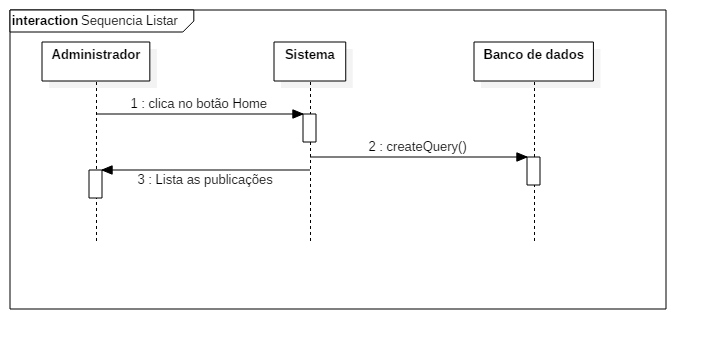
\includegraphics[width=\textwidth]{figuras/sequenciaListar}
    \caption{Diagrama de sequência para listar}
\end{figure}